\chapter{转动与振动光谱}\label{ch:b3:rovibrational-spectroscopy}

在一处高而干燥的高原上，数十架射电天线正对着一团暗色的
星际云。在它们所接收的频率中，有一个位于
\qty{115.271}{GHz}：一氧化碳分子处于几开尔文的低温下，
从第一转动激发能级跃迁至最低能级。由这一个数值，化学家
即可求得精确到皮米几分之一的 C–O 键长；由
其后谱线的强度可得该云团的温度。本章
讨论分子的转动与振动：其
能级取自
\cref{ch:b3:quantum-model-systems}中的转子与振子；选择定则取自
\cref{ch:b3:group-theory-applied}；以及光谱所测定的——键长
、力常数与解离能。

\begin{recall}
\Cref{ch:b3:quantum-model-systems}给出了刚性转子，$E_J = J(J+1)\hbar^2/2I$
简并度为 $2J + 1$，以及谐振子 $E_v = (v + \frac12)h\nu$，
对于约化质量为 $\mu$ 的双原子分子。\Cref{ch:b3:group-theory-applied}给出了
红外与拉曼选择定则。本科一年级分册以波数测定了红外
光谱，并定义了分子的极化率。
\end{recall}

\begin{omfigure}
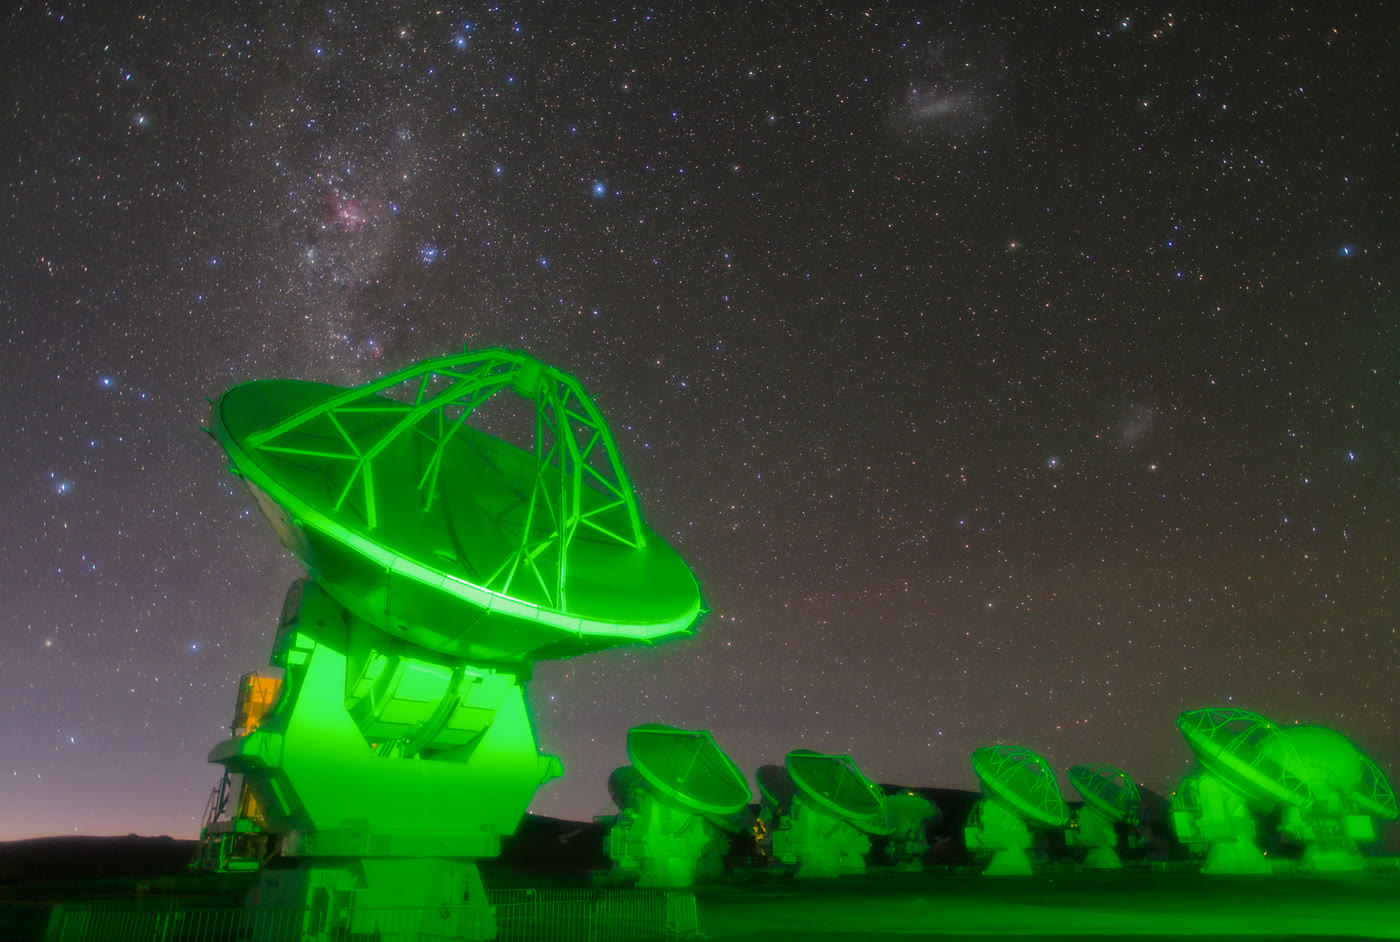
\includegraphics[width=0.7\linewidth]{images/book4/alma-antennas.jpg}

{\small 高原上射电干涉仪的天线，它们记录了众多信号，
其中包括来自星际
云团的一氧化碳转动谱线。摄影：ESO/B.~Tafreshi（twanight.org），CC BY 4.0。}
\end{omfigure}

\section{转动光谱}

\begin{definition}[转动常数、同位素异构体]\label{def:b3:rovibrational-spectroscopy:rotational-constant}
线型分子的\emph{转动常数}\index{转动常数}
为 $B = h/(8\pi^2cI)$，以 \unit{cm^{-1}} 计（或以赫兹计为 $B = h/8\pi^2I$），使其
转动能级以波数计为 $F(J) = BJ(J+1)$。若两分子仅
原子的同位素不同，则互为\emph{同位素异构体}\index{同位素异构体}
（\ce{^{12}C^{16}O}，\ce{^{13}C^{16}O}）；在玻恩–奥本海默近似下，
它们具有相同的键长与力常数。
\end{definition}

\begin{definition}[总选择定则与具体选择定则]\label{def:b3:rovibrational-spectroscopy:selection}
\emph{总选择定则}\index{总选择定则}指出
分子须具有何种性质才能呈现某类光谱；
\emph{具体选择定则}\index{具体选择定则}则指出
哪些量子数的变化是允许的。
\end{definition}

\begin{proposition}[纯转动光谱]\label{prop:b3:rovibrational-spectroscopy:rotational-lines}
分子具有纯转动（微波）光谱，当且仅当其具有
永久偶极矩；对于线型分子，具体选择定则为 $\Delta J
= \pm1$。吸收谱线位于
\[
\tilde\nu = F(J+1) - F(J) = 2B(J + 1), \qquad J = 0, 1, 2, \dots,
\]
间隔相等，均为 $2B$。
\end{proposition}

\begin{proof}
分子与光的相互作用通过偶极矩实现：无
永久偶极矩的分子转动时没有振荡偶极。规则 $\Delta J
= \pm1$ 源自积分 $\int Y_{J'M'}^*\cos\theta\,Y_{JM}$ 在 $J' = J
\pm 1$ 之外均为零（偶极沿 $z$ 的分量按 $Y_{1,0}$ 变换），在本阶段不加证明地承认。
于是 $B(J+1)(J+2) - BJ(J+1) = 2B(J+1)$。
\end{proof}

\begin{method}[由转动谱线求键长]\label{met:b3:rovibrational-spectroscopy:bond-length}
\begin{enumerate}
  \item 由 $J + 1 \leftarrow J$ 的谱线（频率为 $\nu$），求得 $B =
        \nu/2(J+1)$（以赫兹计）。
  \item 计算转动惯量 $I = h/8\pi^2B$。
  \item 由同位素质量求约化质量，则 $r = \sqrt{I/\mu}$。
\end{enumerate}
\end{method}

\begin{example}[一氧化碳]\label{ex:b3:rovibrational-spectroscopy:co}
% ledger: rotl:CO.1-0, imass:O16
谱线 $J = 1 \leftarrow 0$ 属于 \ce{^{12}C^{16}O}，位于 \qty{115271.20}{MHz}：
$B = \qty{57635.6}{MHz} = \qty{1.92252}{cm^{-1}}$, $I = \qty{1.4560e-46}{kg.m^2}$.
取 $\mu = 12 \times 15.99491/27.99491 = \qty{6.85621}{u}$，则 $r_0 = \qty{113.09}{pm}$。
此 $r_0$ 为键在其零点振动上的平均值，略
大于平衡键长 $r_e$（见\cref{sec:b3:rovibrational-spectroscopy:real-bonds}）。
\end{example}

\begin{definition}[离心畸变常数]\label{def:b3:rovibrational-spectroscopy:centrifugal}
转动的键会伸长，能级变为 $F(J) = BJ(J+1) - DJ^2(J+1)^2$，
其中 $D$ 为\emph{离心畸变常数}\index{离心畸变常数}，
而谱线 $2B(J+1) - 4D(J+1)^3$ 在
较高的 $J$ 处缓慢收拢。
\end{definition}

\begin{proposition}[最强谱线]\label{prop:b3:rovibrational-spectroscopy:jmax}
若谱线强度遵循低能级的布居数，此布居数为 $(2J+1)
\eu^{-hcBJ(J+1)/kT}$，则布居最多的能级近似为
\[
J_{\max} \approx \sqrt{\frac{kT}{2hcB}} - \frac12.
\]
\end{proposition}

\begin{proof}
将 $J$ 视为连续变量并求导：$\frac{\dd}{\dd J}[(2J+1)\eu^{-aJ(J+1)}]
= [2 - a(2J+1)^2]\eu^{-aJ(J+1)}$ 其中 $a = hcB/kT$；导数在 $(2J + 1)^2 =
2/a$ 时为零。
\end{proof}

\begin{omfigure}
\begin{tikzpicture}
\begin{axis}[width=0.9\linewidth, height=4.8cm, xmin=0, xmax=70, ymin=0,
  ymax=1.12, ytick=\empty, axis x line=bottom, axis y line=left, ycomb,
  xlabel={波数 / cm$^{-1}$}, ylabel={相对强度},
  tick label style={font=\small}, label style={font=\small}]
\addplot[omDef, very thick] table[x=nu, y=I] {figdata/out/bachelor-3-rotational-spectrum-co-30.dat};
\addplot[omThm, thick, xshift=1.2pt] table[x=nu, y=I] {figdata/out/bachelor-3-rotational-spectrum-co-300.dat};
\end{axis}
\end{tikzpicture}

{\small 一氧化碳的转动吸收光谱，谱线间距
为 $2B = \qty{3.845}{cm^{-1}}$，强度取为较低能级的布居数，
分别在 \qty{30}{K}（蓝色）和 \qty{300}{K}（红色，为便于看清而略作平移）下，
各温度下的强度均按其最强谱线归一化。在 \qty{30}{K} 时最强谱线为
$J = 3 \leftarrow 2$；在 \qty{300}{K} 时为 $J = 8 \leftarrow 7$。}
\end{omfigure}

\section{真实化学键的振动}\label{sec:b3:rovibrational-spectroscopy:real-bonds}

真实化学键在远离平衡位置时不服从胡克定律：
拉伸时它会变软，直至断裂。

\begin{definition}[莫尔斯势]\label{def:b3:rovibrational-spectroscopy:morse}
称\emph{莫尔斯势}\index{莫尔斯势}为 $V(r) = D_e[1 -
\eu^{-\beta(r - r_e)}]^2$：在 $r_e$ 附近近似为谐振子（力常数 $2\beta^2D_e$），
且趋于解离极限 $D_e$（当 $r$ 很大时）。
\end{definition}

\begin{proposition}[莫尔斯振子的能级]\label{prop:b3:rovibrational-spectroscopy:morse-levels}
以波数表示，莫尔斯振子的振动能级为
\[
G(v) = \tilde\omega_e(v + \tfrac12) - \tilde\omega_ex_e(v + \tfrac12)^2, \qquad
\tilde\omega_ex_e = \frac{\tilde\omega_e^2}{4D_e},
\]
能级呈梯状，其横档逐渐靠拢，终止于 $v_{\max} = \lfloor\tilde\omega_e/
2\tilde\omega_ex_e - \frac12\rfloor$。
\end{proposition}
\admitted

莫尔斯方程的求解在更高级的课程中讨论；
能级在本章的图形数据中以数值方式核对。

\begin{definition}[非谐性常数、基频跃迁、泛频、热带]\label{def:b3:rovibrational-spectroscopy:anharmonic}
$\tilde\omega_ex_e$ 称为\emph{非谐性常数}\index{非谐性常数}。
\emph{基频跃迁}\index{基频跃迁}为
$v = 1 \leftarrow 0$；\emph{泛频}\index{泛频}为 $v = n \leftarrow 0$，
其中 $n \ge 2$ 时强度较弱，原因是谐振子的总选择定则 $\Delta v = \pm1$
仅被轻微打破；\emph{热带}\index{热带}起始于
激发态能级，如 $v = 2 \leftarrow 1$，且其强度随温度升高而增大。
\end{definition}

\begin{definition}[光谱解离能]\label{def:b3:rovibrational-spectroscopy:dissociation}
分子的\emph{光谱解离能}\index{光谱解离能}
即其势能的深度 $D_e$，从极小值点量起，
或从最低能级量得的 $D_0 = D_e - G(0)$——
指每个分子在 \qty{0}{K} 下的值，不同于本科二年级分册中的键解离焓，
后者为 \qty{298}{K} 时的摩尔焓。
\end{definition}

\begin{corollary}[莫尔斯振子的 $D_e$ 与 $D_0$]\label{cor:b3:rovibrational-spectroscopy:de}
$D_e = \tilde\omega_e^2/4\tilde\omega_ex_e$ 和 $D_0 = D_e - (\frac12\tilde\omega_e -
\frac14\tilde\omega_ex_e)$。
\end{corollary}

\begin{proof}
前者即命题中的关系式，后者为 $G(0)$。
\end{proof}

\begin{proposition}[伯奇–斯波纳外推法]\label{prop:b3:rovibrational-spectroscopy:birge-sponer}
相邻能级的间距 $\Delta G(v + \frac12) = G(v+1) - G(v) = \tilde\omega_e - 2\tilde\omega_ex_e(v +
1)$ 随 $v$ 线性减小；将它们求和直至为零，即得 $D_0$，
即 $\Delta G$ 对 $v$ 作图的曲线下面积。
\end{proposition}

\begin{proof}
将 $G$ 的两个表达式相减。$D_0$ 为从 $v = 0$ 到
极限的能量，即所有间距之和。
\end{proof}

\begin{example}[氯化氢]\label{ex:b3:rovibrational-spectroscopy:hcl}
% ledger: diat:HCl.we, diat:HCl.wexe, janaf:H.dfH0, janaf:Cl.dfH0, janaf:HCl.dfH0
对 \ce{H^{35}Cl}，$\tilde\omega_e = \qty{2990.95}{cm^{-1}}$ 和 $\tilde\omega_ex_e =
\qty{52.82}{cm^{-1}}$，基频位于 $\tilde\omega_e - 2\tilde\omega_ex_e =
\qty{2885.3}{cm^{-1}}$，第一泛频位于 $2\tilde\omega_e - 6\tilde\omega_ex_e =
\qty{5665.0}{cm^{-1}}$，略小于基频的两倍。莫尔斯模型
给出 $D_e = \qty{42342}{cm^{-1}}$ 和 $D_0 = \qty{40860}{cm^{-1}}$；真实的 $D_0$，
由 H、Cl 与 HCl 在 \qty{0}{K} 时的生成焓得到，为
\qty{35760}{cm^{-1}}（\qty{4.43}{eV}）。真实势能趋于平坦的速度比
在势阱底部拟合的莫尔斯曲线更快，由较低能级作伯奇–斯波纳外推
所得解离能往往被高估。
\end{example}

\begin{omfigure}
\begin{tikzpicture}
\begin{axis}[name=morse, width=0.55\linewidth, height=6cm, xmin=0.8, xmax=4.0,
  ymin=0, ymax=48000, axis lines=left, xlabel={$r$ / \AA}, ylabel={$V$ / cm$^{-1}$},
  unbounded coords=jump, scaled y ticks=false, ytick={0,10000,20000,30000,40000},
  tick label style={font=\small}, label style={font=\small}]
\addplot[black, thick] table[x=r, y=V] {figdata/out/bachelor-3-morse-levels.dat};
\addplot[gray, dashed] table[x=r, y=harm] {figdata/out/bachelor-3-morse-levels.dat};
\addplot[omDef] table[x=r, y=E] {figdata/out/bachelor-3-morse-levels-levels.dat};
\draw[<->, omThm] (axis cs:3.7,0) -- (axis cs:3.7,42342) node[pos=0.5, left, font=\small] {$D_e$};
\draw[dashed, omThm] (axis cs:1.2,42342) -- (axis cs:4.0,42342);
\end{axis}
\begin{axis}[at={(morse.east)}, anchor=west, xshift=1.6cm, width=0.4\linewidth,
  height=5cm, xmin=0, xmax=28, ymin=0, ymax=3100, axis lines=left,
  xlabel={$v$}, ylabel={$\Delta G(v + \frac12)$ / cm$^{-1}$},
  tick label style={font=\small}, label style={font=\small}]
\addplot[omDef, only marks, mark size=1.2pt] table[x=v, y=dG] {figdata/out/bachelor-3-morse-levels-bs.dat};
\addplot[omDef!40, fill=omDef!12, draw=none] table[x=v, y=dG] {figdata/out/bachelor-3-morse-levels-bs.dat} \closedcycle;
\end{axis}
\end{tikzpicture}

{\small 左图：由 \ce{HCl} 的光谱常数构造的莫尔斯势
（实线）、同曲率的谐振子抛物线（虚线），
以及每第三个振动能级，各自画在两转折点之间；
能级向 $D_e$ 收拢。右：间距的伯奇–斯波纳图；
阴影面积即 $D_0$。}
\end{omfigure}

\section{振转谱带}

气体的振动跃迁伴随转动的变化，$\Delta
J = \pm1$，对于处于 ${}^1\Sigma$ 态的双原子分子。

\begin{definition}[P 支、Q 支和 R 支；谱带原点]\label{def:b3:rovibrational-spectroscopy:branches}
在振转谱带中，$\Delta J = -1$ 的谱线构成\emph{P
支}\index{P 支}
，$\Delta J = +1$ 的谱线构成\emph{R 支}\index{R 支}，
而 $\Delta J = 0$（若允许）的谱线构成\emph{Q 支}\index{Q 支}。
\emph{谱带原点}\index{谱带原点} $\tilde\nu_0$ 为
不计转动时的振动能量差。
\end{definition}

\begin{theorem}[组合差分]\label{thm:b3:rovibrational-spectroscopy:combination-differences}
设下、上振动能级的转动常数分别为 $B_0$ 和 $B_1$，
则 $R(J) = \tilde\nu_0 + B_1(J+1)(J+2) - B_0J(J+1)$，$P(J) = \tilde\nu_0 +
B_1(J-1)J - B_0J(J+1)$，且
\[
R(J - 1) - P(J + 1) = 4B_0(J + \tfrac12), \qquad R(J) - P(J) = 4B_1(J + \tfrac12).
\]
\end{theorem}

\begin{proof}
前两式由 $E = G(v) + B_vJ(J+1)$ 对两能级分别得出。$R(J - 1)$ 与
$P(J + 1)$ 终止于同一上能级 $J$，分别来自下能级 $J - 1$ 和 $J + 1$：
二者之差为 $B_0[(J+1)(J+2) - (J-1)J] = B_0(4J + 2)$。同理，$R(J)$ 与
$P(J)$ 始于同一下能级，分别终止于 $J + 1$ 和 $J - 1$。
\end{proof}

\begin{method}[分析振转谱带]\label{met:b3:rovibrational-spectroscopy:combination}
\begin{enumerate}
  \item 定出间隙：对于 ${}^1\Sigma$ 双原子分子不存在 Q 支，且
        $\tilde\nu_0$ 位于间隙中，介于 $R(0)$ 与 $P(1)$ 之间。
  \item 从间隙向外给谱线编号：$R(0), R(1), \dots$ 与 $P(1),
        P(2), \dots$。
  \item 利用组合差分别求出 $B_0$ 与 $B_1$，
        再依次算出 $\alpha_e = B_0 - B_1$ 与 $B_e = B_0 + \frac12\alpha_e$。
\end{enumerate}
\end{method}

\begin{omfigure}
\begin{tikzpicture}
\begin{axis}[width=0.92\linewidth, height=5cm, xmin=2650, xmax=3080, ymin=0,
  ymax=1.15, ytick=\empty, axis x line=bottom, axis y line=left,
  xlabel={波数 / cm$^{-1}$}, ylabel={吸光度（相对值）},
  tick label style={font=\small}, label style={font=\small}]
\addplot[omDef, thin] table[x=nu, y=A] {figdata/out/bachelor-3-rovib-band.dat};
\node[font=\small] at (axis cs:2780,1.06) {P 支};
\node[font=\small] at (axis cs:2985,1.06) {R 支};
\draw[->, gray] (axis cs:2885.3,0.45) -- (axis cs:2885.3,0.05);
\node[font=\small, gray, anchor=south] at (axis cs:2885.3,0.45) {$\tilde\nu_0$};
\end{axis}
\end{tikzpicture}

{\small \qty{300}{K} 下气态 \ce{HCl} 的基频谱带，由
其光谱常数算出：间隙位于谱带原点处，两侧为 P 支和 R 支。
每条谱线都是双线，即 \ce{H^{35}Cl} 与较弱、略低的
\ce{H^{37}Cl}（天然丰度分别为 76\,\% 和 24\,\%）。R 支谱线收拢，
P 支谱线散开，因为 $B_1 < B_0$。}
\end{omfigure}

\begin{example}[由谱带求 \ce{HCl} 的常数]\label{ex:b3:rovibrational-spectroscopy:analysis}
% ledger: diat:HCl.Be, diat:HCl.ae
已知 $R(0) = \qty{2905.58}{cm^{-1}}$，$P(2) = \qty{2842.94}{cm^{-1}}$，可得
$6B_0 = \qty{62.64}{cm^{-1}}$，故 $B_0 = \qty{10.440}{cm^{-1}}$。又由 $R(1) = 2925.23$ 与 $P(1) =
\qty{2864.43}{cm^{-1}}$，得 $B_1 = \qty{10.133}{cm^{-1}}$。于是 $\alpha_e = \qty{0.307}{cm^{-1}}$
与 $B_e = \qty{10.593}{cm^{-1}}$，即构造该谱带所用的数值：
该方法恰好复原了这些数值。
\end{example}

\section{拉曼光谱}

\begin{definition}[拉曼散射与瑞利散射]\label{def:b3:rovibrational-spectroscopy:raman}
频率为 $\nu_0$ 的光穿过样品时，大部分散射光
保持频率 $\nu_0$，称为\emph{瑞利散射}\index{瑞利散射}。
一小部分散射光的频率因分子的转动或振动
频率而发生偏移，称为\emph{拉曼散射}\index{拉曼散射}。
频率较低的谱线称为\emph{斯托克斯线}\index{斯托克斯线}（分子
获得能量），频率较高的谱线称为\emph{反斯托克斯线}\index{反斯托克斯线}
（分子失去能量）。
\end{definition}

\begin{proposition}[拉曼效应的经典起源]\label{prop:b3:rovibrational-spectroscopy:raman-classical}
若以 $\nu_{\mathrm{vib}}$ 振动的分子，其极化率
按 $\alpha = \alpha_0 + \alpha_1\cos(2\pi\nu_{\mathrm{vib}}t)$ 变化，则
在场 $E_0\cos(2\pi\nu_0t)$ 作用下诱导的偶极以 $\nu_0$ 及 $\nu_0 \pm \nu_{\mathrm{vib}}$ 振荡。
只有使极化率发生变化的振动才具有拉曼活性。
\end{proposition}

\begin{proof}
$\mu = \alpha E = \alpha_0E_0\cos(2\pi\nu_0t) + \frac12\alpha_1E_0[\cos2\pi(\nu_0 +
\nu_{\mathrm{vib}})t + \cos2\pi(\nu_0 - \nu_{\mathrm{vib}})t]$，由 $\cos a\cos b =
\frac12[\cos(a+b) + \cos(a-b)]$。每个振荡偶极以
自身频率辐射；若无 $\alpha_1$，则只剩瑞利项。
\end{proof}

\begin{proposition}[转动拉曼谱线]\label{prop:b3:rovibrational-spectroscopy:rotational-raman}
具有各向异性极化率的线型分子给出转动拉曼谱线，
谱线满足 $\Delta J = \pm2$，与激发线的偏移为
\[
|\Delta\tilde\nu| = F(J+2) - F(J) = 4B(J + \tfrac32) = 6B, 10B, 14B, \dots
\]
——第一条谱线位于 $6B$，此后间隔为 $4B$。
\end{proposition}

\begin{proof}
线型分子转动时，其极化率椭球每转一周两次回到相同取向，
因此它以转动频率的两倍
调制散射：$\Delta J = \pm2$（量子规则，在本阶段不加证明地承认）。于是
$B(J+2)(J+3) - BJ(J+1) = B(4J + 6)$。
\end{proof}

\begin{example}[用拉曼光谱看氮气]\label{ex:b3:rovibrational-spectroscopy:n2}
% ledger: diat:N2.Be, diat:N2.ae
\ce{N2} 没有偶极矩，也没有红外光谱与微波光谱，但其
极化率各向异性：其转动拉曼谱线距激发线的起点为 $6B_0 =
\qty{11.94}{cm^{-1}}$，相邻谱线间隔为 \qty{7.96}{cm^{-1}}。其
强度在偶数与奇数 $J$ 之间以 2:1 交替：两个 \ce{^{14}N} 核
全同，核自旋统计（见\cref{ch:b3:statistical-thermo-applied}）
使偶数 $J$ 能级的权重为奇数能级的两倍。
\end{example}

\begin{omfigure}
\begin{tikzpicture}
\begin{axis}[name=r, width=0.55\linewidth, height=4.6cm, xmin=-110, xmax=110,
  ymin=0, ymax=1.1, ytick=\empty, axis x line=bottom, axis y line=left, ycomb,
  xlabel={拉曼位移 / cm$^{-1}$}, tick label style={font=\small}, label style={font=\small},
  title={\small \ce{N2}，转动拉曼，\qty{300}{K}}]
\addplot[omDef, thick] table[x=shift, y=I] {figdata/out/bachelor-3-rotational-spectrum-n2-raman.dat};
\draw[gray, thick] (axis cs:0,0) -- (axis cs:0,1.05);
\end{axis}
\begin{scope}[xshift=0.6\linewidth, font=\small]
  \draw[omstate] (0,0) -- (2.4,0) node[right] {$v = 0$};
  \draw[omstate] (0,1.0) -- (2.4,1.0) node[right] {$v = 1$};
  \draw[omvib, densely dashed] (0,3.2) -- (2.4,3.2) node[right] {虚能级};
  \draw[omabs] (0.3,0) -- (0.3,3.18);
  \draw[omfluo] (0.5,3.18) -- (0.5,0.02);
  \node[font=\scriptsize, omThm, anchor=east] at (0.22,1.6) {瑞利};
  \draw[omabs] (1.3,0) -- (1.3,3.18);
  \draw[omphos] (1.5,3.18) -- (1.5,1.02) node[pos=0.4, right, font=\scriptsize] {斯托克斯};
\end{scope}
\end{tikzpicture}

{\small 左图：在
\qty{300}{K} 下计算的氮气转动拉曼谱：斯托克斯线位于正位移处（右侧），反斯托克斯线位于
负位移处（左侧，略弱），强度呈 2:1 交替的
规律；零位处的灰线标出强得多的瑞利线。右图：瑞利散射与斯托克斯散射
经虚能级的能级示意（虚能级并非分子的真实态）。}
\end{omfigure}

\section{多原子分子}

\begin{definition}[转子的类型]\label{def:b3:rovibrational-spectroscopy:rotor-types}
三个主转动惯量均相等的分子，称为
\emph{球陀螺}\index{球陀螺}（\ce{CH4}、\ce{SF6}）；两个相等的，称为
\emph{对称陀螺}\index{对称陀螺}（\ce{NH3}、\ce{CHCl3}、\ce{C6H6}）；
三个都不相等的，称为\emph{不对称陀螺}\index{不对称陀螺}
（\ce{H2O}、多数分子）；线型分子则有一个主转动惯量为零。
\end{definition}

球陀螺没有偶极矩，也没有转动光谱；对称陀螺的
$BJ(J+1) + (A - B)K^2$ 能级，其中 $K$ 表征绕其轴的角动量；
谱线仍落在 $2B(J+1)$ 处，因 $\Delta K = 0$；不对称陀螺
具有不规则的光谱，需用计算机拟合。多原子分子的振动
即其简正模式，其标记与选取见
\cref{ch:b3:group-theory-applied}：红外光谱显示的是
变换为 $x$、$y$、$z$ 的模式，每种模式都有各自的转动结构。

\begin{inthelab}[红外光谱仪中的气体样品池]
将气态 \ce{HCl} 充入 \qty{10}{cm} 的样品池，池窗对红外
透明，置于傅里叶变换光谱仪中。在 \qty{1}{cm^{-1}}
分辨率下，P 支与 R 支各呈单线；在 \qty{0.25}{cm^{-1}}
分辨率下，两支各分裂为各自的 \ce{H^{35}Cl}/\ce{H^{37}Cl} 双峰，相距 \qty{2}{cm^{-1}}。氯化氢
有毒且具腐蚀性：样品池在真空管线上充装，并在通风
橱中操作。
\end{inthelab}

\begin{safety}{\ghs[0.8cm]{GHS04}\ghs[0.8cm]{GHS05}\ghs[0.8cm]{GHS06}}
氯化氢气体：加压气体，可腐蚀皮肤、眼睛和
呼吸道，吸入有毒。仅可在密闭装置或
通风橱中操作。
\end{safety}

\begin{history}[拉曼，1928 年]
1928 年，拉曼与克里希南观察到，阳光经紫色滤光片过滤后
照射液体并被散射，产生一种颜色不同的微弱光，
用与之正交放置的绿色滤光片即可将其分离。拉曼于 1930 年获得
诺贝尔物理学奖；激光光源使其效应成为常规的分析
技术，那已是五十年之后的事。
\end{history}

\section{练习}

\begin{exercise}[$\star$]\label{exo:b3:rovibrational-spectroscopy:1}
% ledger: imass:O16
已知 $B_0 = \qty{1.9225}{cm^{-1}}$，对 \ce{^{12}C^{16}O} 求其
转动惯量和键长 $r_0$。
\end{exercise}

\begin{exercise}[$\star$]\label{exo:b3:rovibrational-spectroscopy:2}
% ledger: diat:HCl.Be, diat:HCl.ae
已知 $B_0 = \qty{10.440}{cm^{-1}}$，求 \ce{H^{35}Cl} 转动光谱前四条谱线的
位置，并给出在
\qty{300}{K} 下最强谱线对应的 $J$ 值。
\end{exercise}

\begin{exercise}[$\star$]\label{exo:b3:rovibrational-spectroscopy:3}
在 \ce{H2}、\ce{HCl}、\ce{N2}、\ce{CO2}、\ce{CH4}、\ce{SF6} 和 \ce{H2O} 中，
哪些呈现纯转动吸收光谱？哪些呈现转动拉曼光谱？
\end{exercise}

\begin{exercise}[$\star$]\label{exo:b3:rovibrational-spectroscopy:4}
% ledger: diat:HCl.we, diat:HCl.wexe
\ce{HCl} 分子处于 $v = 1$ 态的比例，在 300 与 \qty{1000}{K} 时各为多少
（基频 \qty{2885.3}{cm^{-1}}）？热带何时变得可见？
\end{exercise}

\begin{exercise}[$\star\star$]\label{exo:b3:rovibrational-spectroscopy:5}
\ce{H^{35}Cl} 的基频与第一泛频分别位于 2885.3 与
\qty{5665.0}{cm^{-1}} 处。由此求出 $\tilde\omega_e$ 与 $\tilde\omega_ex_e$。
\end{exercise}

\begin{exercise}[$\star\star$]\label{exo:b3:rovibrational-spectroscopy:6}
利用上一题的常数，求莫尔斯模型的 $D_e$ 与 $D_0$，
并与真实值 $D_0 = \qty{35760}{cm^{-1}}$ 比较。将
两个 $D_0$ 均换算为 \unit{kJ/mol}。
\end{exercise}

\begin{exercise}[$\star\star$]\label{exo:b3:rovibrational-spectroscopy:7}
\ce{H^{35}Cl} 基频的四条谱线为 $R(0) = 2905.58$、$R(1) = 2925.23$、
$P(1) = 2864.43$ 与 $P(2) = \qty{2842.94}{cm^{-1}}$。求 $B_0$、$B_1$、$\alpha_e$ 及
谱带原点。
\end{exercise}

\begin{exercise}[$\star\star$]\label{exo:b3:rovibrational-spectroscopy:8}
% ledger: imass:H1, imass:H2, imass:Cl35
预测 \ce{D^{35}Cl} 的 $B_0$ 与谱带原点，由 \ce{H^{35}Cl} 的数据推出，
并利用约化质量间的关系（$\tilde\omega_e \propto \mu^{-1/2}$，$\tilde\omega_ex_e \propto
\mu^{-1}$，$B \propto \mu^{-1}$）。
\end{exercise}

\begin{exercise}[$\star\star$]\label{exo:b3:rovibrational-spectroscopy:9}
% ledger: diat:N2.Be, diat:N2.ae
对 \ce{N2}，$B_0 = \qty{1.9896}{cm^{-1}}$。求前三条
斯托克斯转动拉曼线的位移，并解释它们的
强度交替变化的原因。
\end{exercise}

\begin{exercise}[$\star\star\star$]\label{exo:b3:rovibrational-spectroscopy:10}
% ledger: rotl:CO.1-0, rotl:CO.2-1, rotl:CO.3-2
\ce{^{12}C^{16}O} 的前三条转动谱线位于 115271.2018、
230538.0000 与 \qty{345795.9899}{MHz} 处。证明刚性转子模型不能拟合这些谱线，
并求 $B$ 与离心畸变常数 $D$。
\end{exercise}

\begin{exercise}[$\star\star\star$]\label{exo:b3:rovibrational-spectroscopy:11}
证明莫尔斯振子的伯奇–斯波纳求和，即能级间隔 $\Delta G(v + \frac12)$ 自 $v = 0$
至最后一个束缚态之和近似等于 $D_e - G(0)$，并
对 \ce{HCl} 计算该和值。
\end{exercise}

\begin{exercise}[$\star\star\star$]\label{exo:b3:rovibrational-spectroscopy:12}
\ce{^{16}O} 原子核自旋为零，因此 \ce{^{16}O^{12}C^{16}O} 中
$J$ 为奇数的能级不存在。求其转动拉曼线的间隔，以及
第一条线的位移（用 $B$ 表示）。为何 \ce{CO2} 没有
微波谱？
\end{exercise}

\section{问题：聆听冷云}

\begin{problem}[{周末问题——由一氧化碳的第一条转动谱线求键长、
星际云的温度、
碳-13 同位素异构体与红外谱带}]
\label{pb:b3:rovibrational-spectroscopy:1}
% ledger: rotl:CO.1-0, rotl:CO.2-1, rotl:13CO.1-0, imass:O16, imass:C13, iso:C13, diat:CO.we, diat:CO.wexe, re:CO
数据：\ce{^{12}C^{16}O} 的谱线 $J = 1 \leftarrow 0$ 位于 \qty{115.2712}{GHz}，$2
\leftarrow 1$ 位于 \qty{230.5380}{GHz}；\ce{^{13}C^{16}O} 的 $1 \leftarrow 0$ 谱线位于
\qty{110.2014}{GHz}；质量分别为 \ce{^{12}C} 12（精确值），\ce{^{13}C} 13.00335，
\ce{^{16}O} \qty{15.99491}{u}；\ce{^{13}C} 的天然丰度为 1.1\,\%；对 \ce{^{12}C^{16}O}，
$\tilde\omega_e = \qty{2169.81}{cm^{-1}}$，$\tilde\omega_ex_e = \qty{13.288}{cm^{-1}}$，以及
平衡键长 $r_e = \qty{112.83}{pm}$。$h = \qty{6.62607e-34}{J.s}$，$u =
\qty{1.66054e-27}{kg}$，$c = \qty{2.99792e10}{cm/s}$，$hc/k = \qty{1.43878}{cm.K}$。

\medskip\noindent\textbf{第一部分——键。}
\begin{enumerate}
  \item 以赫兹与 \unit{cm^{-1}} 为单位，求 $B_0$。
  \item 求 \ce{^{12}C^{16}O} 的约化质量，单位为千克。
  \item 求转动惯量。
  \item 由此求 $r_0$。
  \item 与 $r_e$ 比较。为何 $r_0$ 更长？
  \item 对刚性转子预测 $2 \leftarrow 1$ 谱线，并评论
        测量值。
\end{enumerate}

\medskip\noindent\textbf{第二部分——云的温度。}
\begin{enumerate}[resume]
  \item 分别以 \unit{cm^{-1}} 与开尔文（$E/k$）为单位，求能级 $J =
        0$、1、2 的能量。
  \item 写出布居数之比 $N_2/N_1$ 在温度 $T$ 时的表达式。
  \item 观察结果给出 $N_2/N_1 = 0.85$（题中数据）。求 $T$。
  \item 该温度下哪一能级布居数最多？
  \item 为何这样的云在红外振动谱带中无法被观测到？
  \item 为何 $1 \leftarrow 0$ 谱线是最常用的冷气体示踪剂？
\end{enumerate}

\medskip\noindent\textbf{第三部分——同位素异构体。}
\begin{enumerate}[resume]
  \item 求 \ce{^{13}C^{16}O} 的约化质量。
  \item 由 \ce{^{12}C^{16}O} 的谱线预测其 $1 \leftarrow 0$ 谱线。
  \item 与测得的 \qty{110.2014}{GHz} 比较。忽略了什么？
  \item 若两条谱线均弱且未饱和，则天然丰度给出的
        强度之比为多少？
  \item 观测比值远小于此，这对
        \ce{^{12}C^{16}O} 谱线说明了什么？
  \item 实际中为何两种同位素异构体往往一起被观测？
\end{enumerate}

\medskip\noindent\textbf{第四部分——振动谱带。}
\begin{enumerate}[resume]
  \item 求基频的谱带原点，分别以 \unit{cm^{-1}} 与
        微米为单位。
  \item 求第一泛频。
  \item 求零点能。
  \item 是什么将第一条 R 支与第一条 P 支谱线分开？
  \item 在 \ce{^{12}C^{16}O} 与 \ce{^{13}C^{16}O} 中，哪一个分子的谱带原点更低？
  \item 给出结论：一氧化碳的键长 $r_0$，由
        一条射电谱线求得。
\end{enumerate}
\end{problem}
